\documentclass[a4paper,11pt]{article}

\usepackage{amsmath, amssymb, amstext, amsfonts, mathrsfs}


% \sffamily %schrift ohne Serifen

\usepackage[T1]{fontenc} 
% schriftencodierung f�r umlaute, trennung
% f\"ur Uni
\usepackage[ansinew]{inputenc}
\usepackage{selinput}
% \usepackage[utf8]{inputenc} 
\usepackage{bibgerm} 
% german bibliography
\usepackage[german]{babel}
%wichtig f�r deutschen Content
\usepackage{ucs}
%erweiterte UTF-8 Unterst�tzung
\usepackage{wrapfig} 
% Paket zur Positionierung einbinden
\usepackage{multirow}
% zusammenfassen von Tabellenzellen
% \usepackage{subscript}
% zum tiefstellen
\usepackage{lscape}
\usepackage{pdflscape}
% zum drehen der Seite
% \usepackage[super]{natbib}
\usepackage[square,sort,comma,numbers]{natbib}
% Erstellung es Literaturverzeichnisses
\usepackage{url}
% Umbruch f�r URL
\usepackage{pst-3dplot}
% f�r tex Grafiken n�tig
\usepackage{pstricks}
\usepackage{listings}
% f�r das einf�gen von Quelltext
\definecolor{codegray}{rgb}{0.92,0.92,0.92}
\lstset{basicstyle=\fontsize{9}{11}\selectfont\ttfamily, breaklines=true, backgroundcolor=\color{codegray}, numbers=left, numberstyle=\tiny, tabsize=4, language=java}
\definecolor{mymauve}{rgb}{0.58,0,0.82}
\definecolor{mygreen}{rgb}{0,0.6,0}
\lstset{
commentstyle=\color{mygreen},
keywordstyle=\color{mymauve},
language=Java,
stringstyle=\color{blue}
}


%Einstellungen f�r Quellcode
\usepackage[a4paper, left=3cm, right=2cm, top=2cm]{geometry}
% Formatierung R�nder
\usepackage[section]{placeins}
% f�r Floatbarriere
\usepackage{color}
%f�r die Verwendung von Farben

\clubpenalty = 10000 
\widowpenalty = 10000
\displaywidowpenalty = 10000
%Verhinderung von Hurenkindern und Schusterjungen
%10000 bedeutet die sie sollen kommplett vermieden werden

\title{Serialisierung von Datenobjekten in JSON zur \"Ubertragung von Objekten aus Energieanwendungen}

\author{Sebastian Rieger}

\pagenumbering{arabic}
%Seitenzahlen(arabische Zahlen)

\setlength{\parindent}{0.25cm} 
%Absatzeinzug �ndern in Zoll
\setlength{\parskip}{0.25cm}
%Absatzabstand
\linespread {1.5}
%Zeilenabstand

% \usepackage{hyperref}
%anklickbare Hyperlinks

%funktioniert nicht bei Fu�noten
\usepackage{graphicx}
\usepackage{graphics}
%f�r einbinden von Grafiken
\usepackage{setspace}
\usepackage{framed}
%f�r Umrandung der Erkl�rung
\usepackage{acronym}
% f�r abk�rzungen
% \usepackage{PSTricks}
\usepackage{epstopdf}
% f�r eps bilder nutze pdflatex --shell-escape this.tex
\usepackage{amssymb}
% f�r mathematische Symbole

\usepackage{hyperref}
% klickbare links

% \usepackage{pdfpages}
\usepackage{rotating}
%%%%%%%%%%%%%%%%%%%%%%%%%%%%%%%%%%%%%%%%%%%%%%%%%%%%%%%%%%%%%%%%%%%%%%%%%%%%%%%%%%%%%%%%%%%%%%%%%%%%%
%% Angaben zur Arbeit
%%%%%%%%%%%%%%%%%%%%%%%%%%%%%%%%%%%%%%%%%%%%%%%%%%%%%%%%%%%%%%%%%%%%%%%%%%%%%%%

\newcommand{\Autor}{Sebastian Rieger}
\newcommand{\MatrikelNummer}{7406886}
\newcommand{\Kursbezeichnung}{TINF12B1}

\newcommand{\FirmenName}{Karlsruher Institut f�r Technologie (KIT)}
\newcommand{\FirmenStadt}{Karlsruhe}
\newcommand{\FirmenLogoDeckblatt}{{
\includegraphics[width=3cm]{Bilder/kitlogo}}}

% Falls es kein Firmenlogo gibt:
%  \newcommand{\FirmenLogoDeckblatt}{}

% \newcommand{\BetreuerFirma}{Dr.-Ing. Karl-Uwe Stucky}
\newcommand{\BetreuerDHBW}{Dipl. -Inform. Thorsten Schlachter}
\newcommand{\Titel}{Entwicklung einer Android-Applikation f�r die Alarmierung der Einsatzkr�fte der Freiwilligen Feuerwehren}
\newcommand{\AbgabeDatum}{??????????}

\newcommand{\Dauer}{??????????}

% \newcommand{\Abschluss}{Bachelor of Engineering}
\newcommand{\Abschluss}{Bachelor of Science}

\newcommand{\Studiengang}{Angewandte Informatik}
% \newcommand{\Studiengang}{Angewandte Informatik}
\newcommand{\Was}{Studienarbeit}

%%%%%%%%%%%%%%%%%%%%%%%%%%%%%%%%%%%%%%%%%%%%%%%%%%%%%%%%%%%%%%%%%%%%%%%%%%%%%%%%%%%%%%%%%%%%%%%%%%%%% 
%steuervariable
\usepackage{ifthen} %Package f�r if/else
\newboolean{bilder} %Deklaration
\setboolean{bilder}{true} %Zuweisung
% \setboolean{bilder}{false} %Zuweisung
%%%%%%%%%%%%%%%%%%%%%%%%%%%%%%%%%%%%%%%%%%%%%%%%%%%%%%%%%%%%%%%%%%%%%%%%%%%%%%%%%%%%%%%%%%%%%%%%%%%%%

\begin{document}

\begin{center}
\vspace*{-2cm}
\FirmenLogoDeckblatt\hfill
\includegraphics[width=4cm]{Bilder/dhbw-logo}\\[1cm]
{\Huge \Titel}\\[2cm]
{\Huge\scshape \Was}\\[2cm]
{\large f�r die Pr�fung zum}\\[0.5cm]
{\Large \Abschluss}\\[0.5cm]
{\large des Studienganges \Studiengang}\\[0.5cm]
{\large an der}\\[0.5cm]
{\large Dualen Hochschule Baden-W�rttemberg Karlsruhe}\\[0.5cm]
{\large von}\\[0.5cm]
{\large\bfseries \Autor}\\[1cm]
{\large Abgabedatum \AbgabeDatum}
\vfill
\end{center}
\begin{tabular}{l@{\hspace{1cm}}l}
Bearbeitungszeitraum             & \Dauer                       \\
Matrikelnummer                   & \MatrikelNummer              \\
Kurs                             & \Kursbezeichnung             \\
Ausbildungsfirma                 & \FirmenName                  \\
                                 & \FirmenStadt                 \\
% Betreuer der Ausbildungsfirma    & \BetreuerFirma               \\
Gutachter der Studienakademie    & \BetreuerDHBW                \\
\end{tabular}

\newpage
%Seitenumbruch
%%%%%%%%%%%%%%%%%%%%%%%%%%%%%%%%%%%%%%%%%%%%%%%%%%%%%%%%%%%%%%%%%%%%%%%%%%%%%%
%% Descr:       Vorlage für Berichte der DHBW-Karlsruhe, Erklärung
%% Author:      Prof. Dr. Jürgen Vollmer, vollmer@dhbw-karlsruhe.de
%% $Id: erklaerung.tex,v 1.2 2010/07/22 13:30:27 vollmer Exp $
%%%%%%%%%%%%%%%%%%%%%%%%%%%%%%%%%%%%%%%%%%%%%%%%%%%%%%%%%%%%%%%%%%%%%%%%%%%%%%%

% In Bachelorarbeiten muss eine schriftliche Erklärung abgegeben werden. In allen anderen
% Arbeiten entf�llt diese. Hierin best�tigen die Studierenden, dass die Bachelorarbeit
% selbst�ndig verfasst und s�mtliche Quellen und Hilfsmittel angegeben sind. Diese Erkl�rung
% bildet das zweite Blatt der Arbeit. Der Text dieser Erkl�rung muss auf einer separaten Seite
% wie unten angegeben lauten.

\newpage
\thispagestyle{empty}
\begin{framed}
\begin{center}
\Large\bfseries Erkl\"arung
\end{center}

\noindent
Gem\"a\ss{}�16 (3) der "`Studien- und Pr\"ufungsordnung f\"ur den Studienbereich
Technik"' vom 1.11.2007.

\medskip
\noindent
Ich habe die vorliegende Arbeit selbstst\"andig verfasst und
keine anderen als die angegebenen Quellen und Hilfsmittel verwendet.

\vspace{3cm}
\noindent
\underline{\hspace{4cm}}\hfill\underline{\hspace{6cm}}\\
Ort~~~~~Datum\hfill Unterschrift\hspace{4cm}
\end{framed}

%%%%%%%%%%%%%%%%%%%%%%%%%%%%%%%%%%%%%%%%%%%%%%%%%%%%%%%%%%%%%%%%%%%%%%%%%%%%%%%
\endinput
%%%%%%%%%%%%%%%%%%%%%%%%%%%%%%%%%%%%%%%%%%%%%%%%%%%%%%%%%%%%%%%%%%%%%%%%%%%%%%%

\newpage
\begin{spacing}{0.9}

%Einf�gen Inhaltsverzeichnis
\tableofcontents
\newpage
\section{Einleitung}
Es gibt heute verschiedene M�glichkeiten, die Einsatzkr�fte der Freiwilligen Feuerwehren im Einsatzfall zu alarmieren, wobei die beste und schnellste M�glichkeit einen Alarm abzusetzen, die Verwendung von Funkmeldeempf�ngern ist. Jedoch haben vor allem kleine St�dte und Gemeinden nicht die finanziellen M�glichkeiten, jede Einsatzkraft mit einem dieser Ger�te auszustatten, da nicht nur ihre Anschaffung, sondern auch die Wartung und Reparatur sehr teuer sind. 

Aus diesem Grund wird, vor allem im l�ndlichen Bereich, noch oft auf eine Luftsirene gesetzt, da hier alle Kr�fte mit einem einzigen nicht wartungsaufw�ndigen Ger�t alarmiert werden k�nnen. Doch auch hier ergeben sich viele Nachteile. So sind zum einen Beschallungspl�ne st�ndig fort�zuschreiben, was haupts�chlich durch Neubauten geschuldet ist. Gegebenenfalls muss dann der Standort der Sirene ver�ndert oder weitere angeschafft werden, um eine komplette Abdeckung zu gew�hrleisten. Weiterhin machen neue Baubestimmungen eine Alarmierung zusehends schwerer, da zum Beispiel doppelt oder dreifach verglaste Fenster die Au�enger�usche extrem d�mpfen.

Eine weitere M�glichkeit, den Einsatzkr�ften Bescheid zu geben, ist die der SMS-Alarmierung. Im Einsatzfall wird jedem Mitglied der Feuerwehr eine SMS gesendet. Diese Variante ist sehr kosteng�nstig f�r St�dte und Gemeinden, da nicht spezielle Empf�nger angeschafft werden m�ssen. Denn in der heutigen Zeit hat praktisch jeder ein Smartphone in seinem Besitz. Nachteilig hier ist, dass nicht jeder Nutzer sein Ger�t im h�rbaren Modus betreibt und somit einen Alarm eventuell nicht mitbekommt. 

Da die SMS von einen Server gesendet wird, gibt es keine Absender-Nummer, sondern nur einen String als Absender. Hieraus ergeben sich weitere Nachteile. Zum einen kann kein spezieller Ton hinzuf�gen werden (nummerabh�ngiger Ton), da die ankommende SMS keine Absender-Nummer besitzt und zum anderen ist es bei nahezu allen Ger�ten nicht m�glich, den Lautlos-Modus bei bestimmten Nummern auszusetzen und trotz der stillen Benachrichtigung einen Ton zu spielen. Hierf\"ur muss Abhilfe geschaffen werden, denn eine Alarm-SMS ist von besonderer Wichtigkeit und sollte auf jeden Fall wahrgenommen werden.

Mit Hilfe einer mobilen Applikation k�nnten die genannten Nachteile einer freien SMS-Alarmierung aufgehoben werden. Auf dem freien Markt gibt es schon einige Applikationen, die diese Aufgabe erf�llen, doch sind diese immer an spezielle Benachrichtigungssysteme gebunden, welche teuer lizenziert werden.

F\"ur die Einsatzkr\"afte der Feuerwehr, sowie f\"ur St\"adte und Gemeinden, w\"are es sinnvoll eine lizenzkostenfreie Applikation zur Verf\"ugung zu haben. Dies w\"urde nicht nur Kosten sparen, sondern im Ernstfall sogar Leben retten, da die Einsatzkr\"afte zuverl\"assig \"uber einen Einsatz informiert werden und zu Hilfe eilen k\"onnen.

Da das mobile Betriebssystem Android mit circa 84,6 Prozent Marktanteil am h\"aufigsten anzutreffen ist, soll die Applikation auf diesem Betriebssystem aufsetzen. Eine Adaption der Applikation auf "`iOS"' und "`Windows Phone"' ist zwar angedacht, wird aber im Zuge dieser Arbeit nicht umgesetzt. \cite{GolemMobileBetriebssystem}

\newpage
\section{Aufgabenstellung}
Mit Hilfe einer mobilen Android-Applikation sollen Feuerwehreinsatzkr�fte durch eine eingehende "`Alarm-SMS"' benachrichtigt werden, welche von Leitstellen selbst oder von Privatfirmen stammt, welche die Funkinformationen der Leitstellen auswerten. Die gesendeten SMS sind allerdings nicht als Alarmmeldung sofort identifizierbar, sondern kommen wie jede andere SMS beim Empf�nger an.
Beim Erhalt einer solchen SMS soll der Nutzer des Telefons akustisch �ber einstellbare Klingelt�ne sowie visuell �ber das in Android-Ger�ten �bliche "`Notification-Light"' informiert werden.

Eine Alarm-SMS besteht, wie jede andere SMS auch, zum einen aus dem Absendernamen, welcher eine Telefonnummer oder eine Zeichenkette sein kann. Zum anderen enth�lt die SMS einen Nachrichtentext, in welchem bestimmte Informationen, wie Name der Feuerwehr, Einsatzzeit und Einsatzstichwort stehen.

Um eine Unabh�ngigkeit vom Absendesystem zu erreichen, soll der Nutzer zuerst eine beliebige Zeichenfolge eingeben, auf welche die SMS gepr�ft wird. Hierf�r muss ein Dienst entwickelt werden, welcher jede eingehende SMS pr�ft.

Sollte es sich um eine Alarm-SMS handeln, so soll der Nutzer umgehend darauf besonders hingewiesen werden. Hierf�r soll �berpr�ft werden, welche M�glichkeiten f�r eine besondere Alarmierung im Android-System bestehen.

Der Nutzer soll �ber ein neutrales Regelbasiertes System neue Regeln definieren, diese bearbeiten und l�schen k�nnen. 
Hierf\"ur muss ein System ausgearbeitet werden, welches funktional und nutzerfreundlich ist. Auch soll der Export beziehungsweise der Import von Regeln m\"oglich sein, um diese untereinander austauschen zu k\"onnen.

% Bsp: Absender-Nummer.equals("+4972160825769") AND SMS.getContent().contains("foo")
% ==> Action.Klingelton("Mambo5")
Ein weiteres wichtiges Ziel des zu entwickelnden Systems ist, dass es sich bei einem Neustart des Smartphones automatisch mit dem System startet und somit umgehend, ohne Aktion vom Nutzer, einsatzbereit ist.
F�r diesen Zweck m\"ussen die eingegebenen Regeln gespeichert werden. Hierf�r bietet sich zum einen die Speicherung in einer Datei an, aber auch die Speicherung in einer Datenbank soll in Betracht gezogen werden, da mit ihrer Hilfe auch eine Statistik �ber Eins�tze gemacht werden kann.
Zus�tzlich sollen verschiedene Alarmt�ne zur Auswahl stehen, unter denen der Nutzer w�hlen kann.

Zus\"atzlich zur eigentlichen Alarmierungsfunktion soll untersucht werden, wie sich eine Post-Funktion f\"ur "`Social Networks"' wie Twitter, Facebook oder Google+ umsetzen l\"asst. Sollte sich ein String mit dem Einsatzort in der SMS befinden, so soll die Applikation die M\"oglichkeit bieten eine Navigation zu starten.

Zum Abschluss soll untersucht werden, wie es m\"oglich ist eine SMS oder beziehungsweise eine E-Mail zu senden, um den Einheitsf\"uhrer \"uber ein m\"ogliches kommen beziehungsweise ein Fernbleiben zu melden.


\newpage
\section{Android - eine offene und mobile Plattform}
Android ist ein Betriebssystem, welches erstmals im November 2007 von Google, im Zuge der Ver\"offentlichung, des Android \ac{SDK} vorgestellt wurde. Das Betriebssystem bassiert auf dem Linux-Kernel und wird von der \ac{OHA} entwickelt. Es ist auf Ger\"aten wie Netbooks, Smartphones, Mobiltelefonen und Digitalkameras zu finden und Heute weit Verbreitet. \cite{Kuehn12}

\subsection{Android im Wandel der Zeiten}
\begin{wrapfigure}{r}{4,95cm}
\vspace{-13pt}
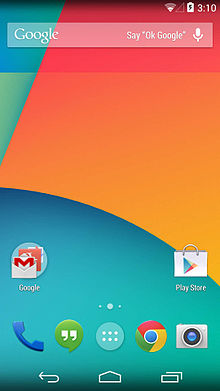
\includegraphics[width=4.95cm]{Bilder/Android4.jpg}
\caption{Android 4.4 Startbildschirm des Nexus 5 in Originalgr\"o\ss{}e \cite{WikiAndroid}}
\label{Der MongoDB-Chooser-Dialog}
\vspace{-20pt}
\end{wrapfigure}
Nach der Ver\"offentlichung des Android \ac{SDK} wurde 2008 mit dem "`G1"' das erste Smartphone mit dem neuen Betriebssystem Android vorgestellt. Ein direkten Vergleich zwischen Android und den von Apple stammenden iOS ging, zu dieser Zeit, klar zu Gunsten der Apple-Produkte aus.
% 
% Dem zu der Zeit noch Marktbeherschenden iOS und den iPhones, konnte 
 
Durch eine schnelle und konsequente Entwicklung konnten, der Firma Apple mit ihrem iOS, immer mehr Marktanteile abgenommen werden. Zum heutgen Zeitpunkt ist die Android-Plattform mit fast 85 Prozent Marktanteil im Bereich der Smartphonebetriebssysteme f\"uhrend. \cite{GolemMobileBetriebssystem}

Hardwarehersteller d\"urfen seit einiger Zeit nicht nur die Oberfl\"ache, sondern auch das Betriebssystem an sich auf ihre ganz speziellen Anforderungen anpassen, was zu einer gro\ss{}en Vielfalt der Plattform f\"uhrte. Ein pures unbearbeitetes Android ist zur Zeit nur auf Ger\"aten der "`Nexus-Reihe"' zu finden, welche zwar von verschiedenen Herstellern gebaut aber von Google vermarktet werden. Dies hat zur Folge das Systemupdates, auf Nexus-Ger\"aten, schneller und regelm\"a\ss{}iger zur Verf\"ugung stehen, da keine Anpassungen an den Updates, durch die Hardwarehersteller, vorgenommen werden m\"ussen.

Android ist momentan in der Version 4.4.4 alias "`Kit Kat"' auf dem Markt. Die Versionsnamen von Android sind immer nach einer S\"u\ss{}speise benannt und kommen in alphabetischer Reihenfolge auf den Markt. So folgte auf "`Jelly Bean"' die aktuelle Version Kit Kat. Eine nun schon in der Entwicklervorschau erschienene Version wird also mit "`L"' beginnen, weshalb diese Version momentan auch "`Android L"' genannt wird. Gut zu sehen ist, dass auf den Buchstaben J ein K folgte, welcher wiederum vom L abgel\"ost wird. \cite{WikiAndroid} \cite{Jung13}

Zus\"atzlich wurde dem Trend der "`Smartwatches"' folgend, im M\"arz 2014, ein speziell f\"ur Smartwatches angepasstes Android-System ver\"offentlicht, welches "`Android Wear"' hei\ss{}t. In dieser Arbeit wird jedoch nicht weiter auf Android Wear eingegangen, da dieses System nur im Zusammenspiel mit einem Smartphone in der Lage ist SMS zu empfangen. \cite{NextAndroidWear}

\subsection{Die Entwicklungsumgenung f\"ur Android}
Das schon angesprochene \ac{SDK} beinhaltet die folgenden Bestandteile:
\begin{itemize}
 \item Die eigentliche Entwicklungsumgenung mit Plugins
 \item Biblioteken und APIs
 \item Das Android Virtual Device
 \item Den USB-Treiber 
 \item Den SDK-Manager
 \item Das Programm dx
 
\end{itemize}

Nach dem downloaden und installieren der Android \ac{SDK} sind die eben genannten Bestandteile auf dem Rechner vorhanden und im Installationsverzeichnis zu finden. Die meisten Entwickler verwenden die \ac{IDE} Eclipse, f\"ur die eigentliche Programmierarbeit. Die im \ac{SDK} vorhandene Version von Eclipse enth\"alt das Plugin \ac{ADT}, welches viele Werkzeuge f\"ur die Android-Entwicklung mitbringt und welche sp\"ater genauer erl\"autert werden.

Eine andere Version des Android \ac{SDK} das sogenannte "`Android Studio"' bassiert auf der \ac{IDE} "`IntelliJ"'. Android Studio besitzt einige zus\"atzliche Features, wie die erweiterte "`Android Code-Completion"' oder die "`Multiple-APK generation"', welche es erlaubt eine Applikation gleichzeitig f\"ur Android und Android Wear zu erzeugen. Trotz der Vorteile, befindet sich das Android Studio noch in einer Beta-Phase und wird daher f\"ur die Entwicklung der App nicht verwendet. \cite{DevAndroidStudio}

Au\ss{}er der \ac{IDE} beinhaltet das Android \ac{SDK} die aktuellen Bibliotheken und APIs, welche f\"ur die Erstellung einer Applikation ben\"otigt werden. Dies beinhaltet auch Klassen, mit dessen Hilfe die zus\"atzliche Hardware in Android-Ger\"aten, wie das Notification-Light, angesprochen werden kann. Des weiteren ist auch eine lauff\"ahige Version des Androidbetriebssystems, welches f\"ur das Virtual Device ben\"otigt wird, vorhanden.

Das Virtual Device simuliert ein Smartphone am Rechner, auf dem die erstelle Applikation ausgef\"uhrt und getestet werden kann. Hierbei werden vom Virtual Device Debug-Information zur \ac{IDE} \"ubertragen, welche von dort aus angeschaut und ausgewertet werden k\"onnen.

Um eine geschriebene Applikation letztendlich nicht nur auf virtuellen Ger\"aten zu testen wird, unter Windows, ein USB-Treiber ben\"otigt. Dieser Treiber erm\"oglicht es, die Applikation auf ein reales Android-Ger\"at zu \"ubertragen und von dort aus zu Debuggen.
Um dies mit realer Hardware zu Testen, muss im entsprechenden Smartphone die "`Entwickler-Option"' aktiviert werden. Wie dies gemacht wird, wird im Kapitel ????? genauer beschrieben.

Der SDK-Manager ist ein Tool, mit dem die einzelnen Android-Version, Bibliotheken, APIs und Eclipse-Plugin-Versionen verwaltet und aktualisiert werden k\"onnen. Dies ist zum Beispiel hilfreich, wenn man eine Applikation unter verschiedenen Android-Version testen oder lauff\"ahig halten will.

Mit dem Namen dx wird ein Compiler bezeichnet, welcher Javaklassen unter Android lauff\"ahig macht. Mehr hierzu ist im folgenden Abschitt zu finden

\subsection{Dalvik anstelle der Java Virtual Machine}
Da eine Applikation f\"ur Android in Java geschrieben wird, liegt es nahe das auch hier eine virtuelle Maschine genutzt wird, welche ein Programm aus f\"uhrt. Im Android-System ist dies die \ac{DVM}, welche die Applikationen ausf\"uhrt.\cite{Android44}

\"Ahnlich wie die \emph{Java Virtual Machine} arbeitet auch Dalvik. Jedoch mit dem gro\ss{}en Unterschied, das Dalvik vom Google-Entwickler Dan Bornstein erdacht wurde um speziell auf leistungsschwachen mobilen Endger\"aten zu funktionieren.

Dalvik ist speziell daf\"ur entwickelt auf Prozessoren mit ARM-Architektur zu arbeiten, wobei die virtuelle Dalvik Maschine hier, im Gegensatz zur Java VM, in der Lage ist Hardwareregister direkt anzusprechen und zu nutzen. Durch die direkte Kommunikation mit der Hardware ergibt sich eine schnellere Verarbeitung des Codes als unter der Java VM direkt.

In der Theorie ist somit jede Javaklasse die unter Dalvik l\"auft auch unter der Java VM lauff\"ahig. Jedoch ergeben sich, in der Praxis, hier meist Schwierigkeiten durch Ein- und Ausgaben, da sich diese beim PC und Touchscreen grundlegend unterscheiden.

\subsubsection{Das Sandbox Prinzip}
Um Sicherheitsaspekten zu gen\"ugen besitzt Dalvik eine sogenannte Sandbox-Funktion, welche es erm\"oglicht Programme getrennt voneinander ausf\"uhren zu k\"onnen. F\"ur jedes auszuf\"uhrende Programm wird, unter Dalvik, eine neue Runtime-Umgegung erstellt, in der das Programm isoliert von anderen arbeitet. 
Dieses Prinzip wird Sandbox genannt, ja jedes Programm nur in seinem eigenen Sandkasten (Sandbox) "`spielen"' kann.

Dieses Vorgehen bringt sowohl Vorteile als auch Nachteile mit sich. Vorteilhaft ist, dass ein Programm nicht auf ein anderes zugreifen kann und dieses ungewollt ve\"andert, oder Daten aus einer anderen Programmausf\"uhrung abgreift. Gleichzeitig ist dieser Vorteil aber auch ein gro\ss{}er Nachteil, da ein gew\"unschter Austausch von Daten ebenfalls unterbunden wird.
Wie eine Daten\"ubertragen dennoch m\"oglich ist, wird im Kapitel ????? genauer behandelt.

\subsubsection{Von *.java zu *.dex}
Nachdem eine Javaklasse geschrieben wurde muss diese \"uber den Javacompiler (javac) in einen *.class-File umgewandelt werden. Dieser Class-File ist in der Theorie von jeder Java VM ausf\"uhrbar. Da die Klasse jedoch unter Dalvik optimiert laufen soll, muss sie ein weiteres mal Kompiliert werden. Diese zweite Kopilierungsstufe wird von dem schon erw\"ahnten Tool dx \"ubernommen. 
Der Dalvik-Compiler dx wandelt einen Class-File in einen von der \ac{DVM} ausf\"uhrbaren .dex-File um.

Dieser Zusammenhang ist in der Abbildung \ref{JavaZuDex} \"uber der Linie noch einmal zu sehen, da der beschriebene Zusammenhang auf dem Entwicklungsrecher passiert.

\begin{figure}[!ht]
\centering
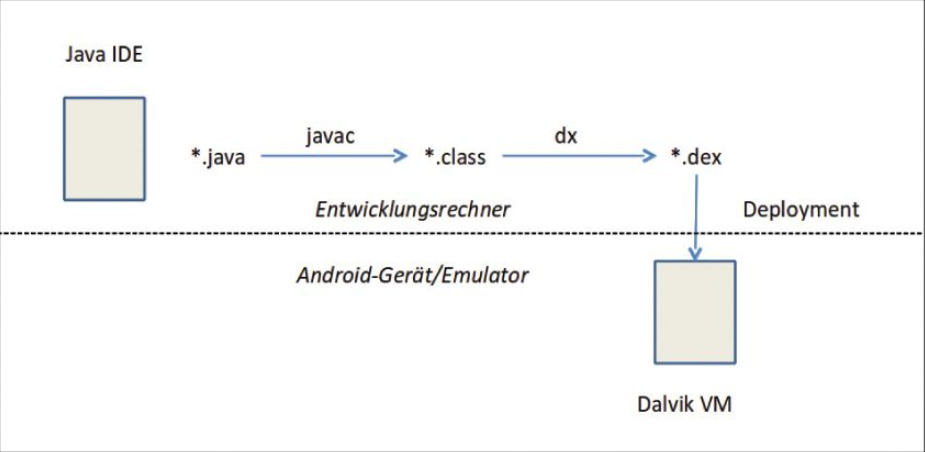
\includegraphics[width=12cm]{Bilder/JavaZuDex}
\caption{Von *.java zu *.dex \cite{Android44}}
\label{JavaZuDex}
\centering
\end{figure}


\end{spacing}




\newpage
\section{Abk�rzungsverzeichnis}
\begin{acronym}
  \acro{SDK}{\emph{Software Development Kits}}
  \acro{OHA}{\emph{Open Handset Alliance}}
  \acro{IDE}{\emph{Integrierte Entwicklungsumgebung}}
  \acro{ADT}{\emph{Android Development Tools}}
  \acro{DVM}{\emph{Dalvik Virtual Machine}}
  \acro{FME}{\emph{Funkmeldeempf\"anger}}
  \acro{JIT}{\emph{Just in Time}}
  \acro{ART}{\emph{Android Runtime}}
  \acro{AOT}{\emph{Ahead-of-Time-Decodierung}}
  \acro{API}{\emph{Application Programming Interface}}
  \acro{}{\emph{}}
%  \acro{KIT}{\emph{Karlsruher Instituts f�r Technologie}}
%  \acro{GDS}{\emph{Generic Data Services}}
% %  \acro{LSDF}{\emph{Large Scale Data Facility}}
%  \acro{OPM}{\emph{Objektorientierten Programmiermodell}}
%  \acro{SMD}{\emph{Strukturelle Metadaten}}
%  \acro{JSON}{\emph{JavaScript Object Notation}}
% %  \acro{HALO}{\emph{High Altitude and Long Range Research Aircraft}}
%  \acro{IAI}{\emph{Institut f�r Angewandte Informatik}}
%  \acro{JAXB}{\emph{Java Architecture for XML Binding}}
%  \acro{UDDE}{\emph{User Data Description Editor}}
%  \acro{AMD}{\emph{Anwendermetadaten}}
%  \acro{CG}{\emph{Class Generator}}
%  \acro{IG}{\emph{Interface Generator}}
\end{acronym}
\newpage
\listoffigures
% Abk�rzungsverzeichnis
\newpage
\bibliographystyle{alphadin}
% verzeichnis im DIN format
\bibliography{Quellen}
\end{document}
